\documentclass[air,article,submit,moreauthors]{Definitions/mdpi}

\firstpage{1}
\makeatletter
\setcounter{page}{\@firstpage}
\makeatother
\pubvolume{1}
\issuenum{1}
\articlenumber{0}
\pubyear{2026}
\copyrightyear{2026}
\datereceived{ }
\daterevised{ }
\dateaccepted{ }
\datepublished{ }

\Title{WRF Cold-Pool Structure and Evolution during a Uinta Basin Winter Ozone Episode}

\newcommand{\orcidauthorA}{0000-0003-0305-4090}
\newcommand{\orcidauthorB}{0009-0009-9083-6568}
\newcommand{\rewritegate}[1]{\textbf{[Rewrite gate: #1]}}
\newcommand{\diagnosticnote}[1]{\textbf{[Diagnostic --- not gate-passed: #1]}}
\newcommand{\exploratorymark}{\textbf{[Exploratory render.]} }
\Author{John R. Lawson $^{1,2,}$*\orcidA{}, Michael J. Davies $^{1}$\orcidB{}, Loknath Dhar $^{1,3}$ and Seth N. Lyman $^{1,3}$}
\AuthorNames{John R. Lawson, Michael J. Davies, Loknath Dhar and Seth N. Lyman}

\address{%
$^{1}$ \quad Bingham Research Center, Utah State University, Vernal, UT 84078, USA;\\
$^{2}$ \quad Department of Mathematics and Statistics, Utah State University, Logan, UT 84322, USA;\\
$^{3}$ \quad Department of Chemistry and Biochemistry, Utah State University, Logan, UT 84322, USA}
\corres{Correspondence: john.lawson@usu.edu}

\abstract{Cold-air-pool structure sets the mixing volume and transport wind that a winter-ozone chemistry model inherits from its meteorological driver, and surface skill alone does not establish it.
We compared four deterministic Weather Research and Forecasting (WRF) simulations of the 2 February 2013 Uinta Basin episode, crossing GFS and NAM driving products with one-way and two-way nest feedback at eleven fixed 1 km station columns over five post-spin-up hours (14:00--18:00 UTC).
Relative to NAM, GFS increased the paired 2 m-temperature-bias contrast by 1.79 and 1.76~$^{\circ}$C under two-way and one-way feedback, reduced 50--500 m stability by 3.63 and 3.65 K, and increased fixed-layer transport wind by 0.79 and 0.99 m s$^{-1}$, with the same sign in all five hours.
Over a registered evaluation footprint, the GFS members also carried 0.70 to 1.80 MJ m$^{-2}$ less integrated heat deficit than the feedback-matched NAM members at every retained hour under seven footprint definitions.
Heat deficit nevertheless increased in every member, so a predeclared test for faster GFS heat-deficit loss failed in all fourteen pair-definition combinations.
Surface-pressure errors ordered the products oppositely, and within-product feedback effects were much smaller throughout.
A matched recomputation of the feedback contrast at the fine-terrain control pair reproduced that bound: every fine-terrain feedback effect was one to two orders of magnitude below the matched driving-product contrast.
Across the controlled archive, the boundary-layer/surface-layer treatment produced a smaller but coherent response, whereas the slope-radiation screen was measurement limited and the fine-terrain-source response failed its predeclared spatial criterion.
This working revision orders those findings by the scientific lever and the strength of its evidence, not by run identifier or completion date; spatial and vertical response structure, terrain-source brackets, and initialization context are retained only with their evidence status explicit.
All five evidence gates of the selected results architecture have been executed with predeclared criteria, and failed gates remain negative results.
The archive design does not separate initial from lateral-boundary forcing, validate inversion depth, establish multi-day persistence, or predict ozone.}

\keyword{winter ozone; WRF; cold-air pool; Uinta Basin; driving data; nest feedback; heat deficit; model evaluation}

\begin{document}

\section{Introduction}

\diagnosticnote{Working-draft mode.
This revision is deliberately broad but selective: it carries every archived controlled comparison and each candidate result thread with a scoped evidential role, while leaving redundant or unreadable figure galleries in the reproducible harvest.
Three status classes appear throughout.
\emph{Promoted} figures and \emph{confirmed} claims have passed the repository's provenance and admission gates and carry ledger identifiers (C-numbers).
\emph{Registered candidates} are tracked with full provenance but are not admitted.
\emph{Exploratory renders} are batch engine figures catalogued in \texttt{figures-draft/HARVEST.md}; they illustrate visual leads only, and no quantitative claim in this draft rests on them.
The analysis gates named in this draft (ANA-17, ANA-18, ANA-19, ANA-20) have all been executed with criteria fixed in committed scripts before any output was read; each section reports its gate's pass or fail outcome, and the complete decision record is \texttt{rewrite/HYBRID-GATE-REVIEW.md}.
A submission-ready revision would remove the remaining diagnostic scaffolding and admit only figures that pass the normal promotion path.}

Winter ozone in the Uinta Basin develops when photochemistry proceeds within snow-covered, stably stratified air that restricts vertical dilution and horizontal exchange \citep{Ahmadov2015-zm,Neemann2015-ws,Davies2025-wy}.
Snow increases actinic flux and modifies deposition, while the stable, weakly ventilated air confines ozone and its precursors near the basin floor.
For a coupled model, the meteorological question is therefore not only whether 2 m temperature has a small mean error.
It is whether the atmosphere delivered to the chemistry grid contains a credible shallow mixing environment and weak transport during the accumulation period.

Published concentration agreement does not provide a clean ranking of the relevant uncertainties.
Ahmadov et al. obtained a much stronger ozone simulation after applying an aircraft-derived, Horsepool-centered emissions scaling while holding the meteorological simulation fixed, and they conditioned the resulting inventory interpretation on adequate meteorology \citep{Ahmadov2015-zm}.
Matichuk et al. evaluated a cumulative ladder that changed volatile-organic-compound emissions, leaf area, and deposition together, while improved WRF temperature profiles did not consistently improve ozone profiles \citep{Matichuk2017-bq}.
These outcomes are consistent with compensating error among confinement, emissions, photolysis, deposition, and chemical mechanism.
They make meteorological evaluation necessary for chemical attribution without making meteorology the uniquely dominant error source.

The meteorological literature also warns against reducing an experiment to a configuration label.
Neemann et al. showed strong case-specific responses from bundled snow, albedo, and cloud-microphysics choices, but their ice-retention modification was a bounding treatment and the 1.33 km grid evaluated most closely was finer than the 4 km meteorology supplied to the chemistry model \citep{Neemann2015-ws}.
Tran et al. showed that the meteorological response to four-dimensional data assimilation depended on the nudged variables, input data, and diagnosed boundary-layer depth; their disclosed artificial formaldehyde limits quantitative chemical inference \citep{Tran2018-ax}.
Thus, labels such as ``NAM driven,'' ``nudged,'' or ``high resolution'' do not by themselves identify a controlled cause, and aggregate scores can obscure a failure to retain the layer of interest.

The archive is not a chronological experiment sequence.
It is a graph of simulations connected by controlled contrasts, and we organize it by the lever that each contrast can identify.
The first question is whether the short-window lower-layer state responds reproducibly to the GFS-versus-NAM driving-data product under both nest-feedback modes.
The second is how the two process treatments represented in the fine-terrain branch---slope-aware radiation and a coupled boundary-layer/surface-layer scheme change---alter that state.
The third is whether the within-product feedback response remains small at both default and fine terrain.
The fourth is whether changing only the static-terrain source produces a coherent basin-floor or terrain-organized response.
For the driving-product contrasts we additionally ask whether the response appears in a footprint-integrated heat-deficit measure and whether the products differ in its within-window change.

Contrasts that share the frozen station and common-height pipeline are displayed together before any individual result is developed.
Terrain-source contrasts instead require area-weighted geometry diagnostics, because a station-only summary can miss a rim- or slope-confined response.
The stable X0--X10 and CMP01--CMP12 codes are retained for provenance, but run numbers do not set manuscript order or evidential weight.
The heat-deficit comparison carries two criteria that were fixed before any output was inspected, and all executed gates retain their pass or fail outcome.
The design evaluates the meteorological input state that a later chemistry calculation would receive; it does not contain a chemistry calculation.

\section{Materials and Methods}

\subsection{Case, Observations, and Evaluation Domains}

The target is the snow-covered Uinta Basin cold-air pool on 2 February 2013 within the episode examined by prior meteorological and chemical studies \citep{Neemann2015-ws,Ahmadov2015-zm}.
All common-sample contrasts use 14:00--18:00 UTC, corresponding to 07:00--11:00 mountain standard time.
The first two forecast hours were excluded as spin-up, leaving five hourly samples; the sensitivity of the results to that two-hour choice has not been evaluated.
Surface observations were extracted from the Synoptic archive for eleven stations reporting 2 m temperature, ten reporting 10 m wind speed, and nine reporting surface pressure in every retained hour.
Subhourly reports were averaged within each UTC clock hour.
The stations span basin-floor, sidewall, and bench locations but are neither spatially uniform nor area weighted.
Every controlled simulation discussed below archived both the 1 km d02 and the 333 m d03 during this window, so output availability did not determine the evaluation domain.
The 1 km d02 was selected for the common observation-linked estimand because it contains all eleven stations, whereas seven stations clamp to the boundary of the roughly 50 by 48 km d03 and only four provide usable interior columns there (ledger row C03).
Figure~\ref{fig:v3-locator} shows the domain geometry, the reporting stations, and the cross-basin transect used by the vertical-section diagnostics.
This coverage decision does not establish that d02 resolves every process response adequately or that a response measured on d02 has the same magnitude or ordering on d03.
The present results therefore describe the full-network d02 sample; a d03 analysis would require a separately declared interior footprint or the same four-station subset on both domains and is not a resolution evaluation.
Four elevation-spanning stations provide surface context from 31 January 00:00 UTC through 4 February 00:00 UTC.
Observed and modeled surface potential temperature for a two-site structural index was calculated as $\theta=T(1000/p)^{0.2854}$, with $T$ in kelvin and $p$ in hPa, and the index was defined as Mountain Home on the northwest bench minus Pariette Draw on the basin floor.
Because the two sites are horizontally separated and locally exposed, the index is a spatial surface contrast rather than a colocated free-air inversion strength or depth.
No sounding, profiler, or remote-sensing profile is used to validate the modeled 50--500 m layer.

\begin{figure}[H]
\centering
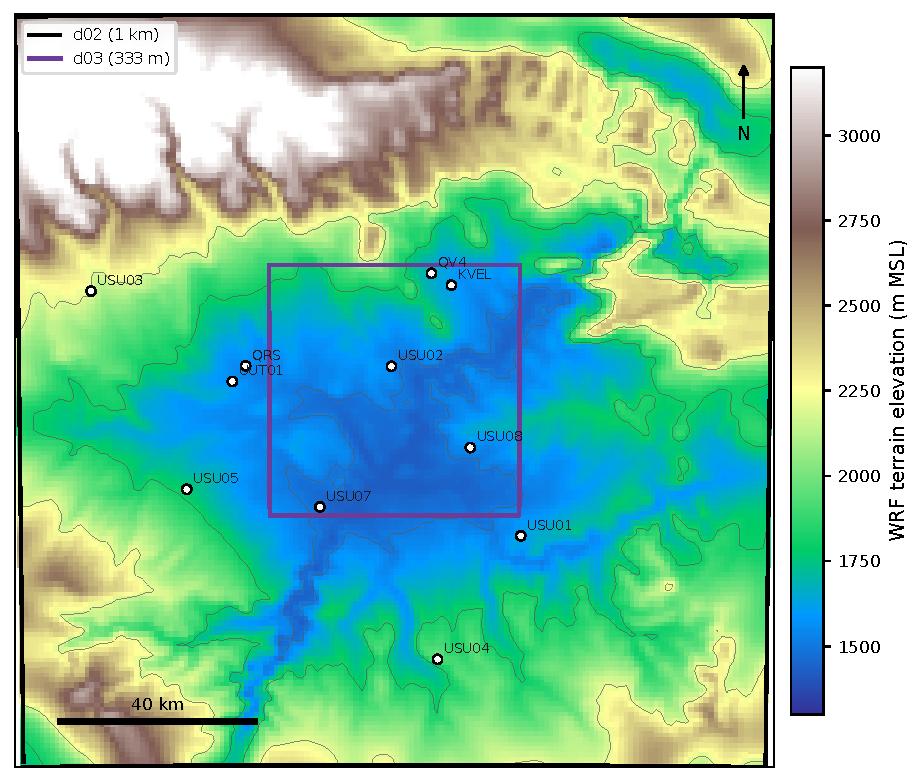
\includegraphics[width=0.78\textwidth]{verification/figures/candidates/wrf_transect_locator_d02_d03.pdf}
\caption{Terrain, reporting stations, and the cross-basin transect on the d02 evaluation domain, with the d03 interior domain outlined.
Registered candidate figure (tracked with full provenance, not promoted).
Seven of the eleven reporting stations fall outside the usable d03 interior, which is why d02 supplies the full-network common sample; the choice does not validate d02 against d03 (C03).}
\label{fig:v3-locator}
\end{figure}

\rewritegate{Synoptic citation wording, the current API defaults, access conditions, and the frozen-cache hash are documented.
Before circulation, archive or regenerate the historical request with explicit quality-control parameters, station and network ownership, sensor metadata, completeness screening, uncertainty treatment, request URL, and provider-specific reuse permission.}

\subsection{WRF Configuration and Archived Simulation Family}
\label{sec:v3-family}

The controlled six-hour simulations used WRF version 4.8.0 from 12:00 to 18:00 UTC on 2 February 2013.
They used three nested domains with horizontal grid spacing of 3, 1, and 0.333 km, 75 eta levels, and a 50 hPa model top.
The reference physics suite used Thompson microphysics, RRTMG longwave and shortwave radiation, the revised MM5 surface layer, the Noah land-surface model, and the YSU planetary-boundary-layer scheme.
Grid and observation four-dimensional data assimilation were disabled.
All deliberate departures from that reference configuration are listed by simulation in Table~\ref{tab:v3-family}.
The GFS one-way member reused the six verified metgrid files from the GFS two-way member before rerunning \texttt{real.exe} and \texttt{wrf.exe}.

\rewritegate{The WRF Version 4 technical reference and v4.8.0 release, GFS grid 004, and NAM grid 218 identities are verified.
Insert only the keys generated by John's small curated bibliography export, and recover the exact input filenames and hashes, map projection, domain dimensions and centers, time step, boundary interval, static-geography versions, and snow-field initialization from the archived as-run records.}

The archive contains eleven stable simulation identifiers, X0--X10 (Table~\ref{tab:v3-family}).
An X code identifies a simulation configuration; it is not itself an experiment or a claim.
Run identity, exact archive paths, namelist fingerprints, and feedback flags are recorded in the run inventory, and directory or figure labels are never used as identity.
As-run differencing connects the controlled family into four scientific branches: driving-data product, boundary-layer and radiation treatments, nest feedback, and static-terrain source.
The X7 and X8 configurations differ from the controlled family in several dimensions at once and enter only as design context (Section~\ref{sec:v3-resolution}).

\begin{table}[H]
\caption{The archived simulation family.
Every run uses WRF 4.8.0, three nests at 3/1/0.333 km with 75 levels, Thompson microphysics, RRTMG radiation, and Noah land surface unless stated.
``Fine terrain'' is a 3-arc-second static source, ``default'' a 30-arc-second-class source, and ``coarse'' a 5-arc-minute source; source resolution is not model-grid spacing.
X7 and X8 are context only: they differ from the controls in several dimensions at once.}
\label{tab:v3-family}
\centering
\small
\begin{tabularx}{\textwidth}{llLL}
\toprule
Code & Product, feedback & Deliberate configuration role & Status \\
\midrule
X0  & NAM, one-way & fine-terrain control, YSU/MM5 & control for X1, X3, X4, X9 \\
X1  & NAM, one-way & X0 plus slope radiation and shading & controlled pair (CMP07) \\
X2  & NAM, one-way & X1 with MYJ/Eta instead of YSU/MM5 & controlled pair (CMP08) \\
X3  & NAM, one-way & default terrain; reference configuration & pairs CMP02, 03, 09, 10 \\
X4  & NAM, one-way & deliberately coarse 5-arc-minute terrain & lineage closed; pairs CMP10, 11 \\
X5  & NAM, two-way & default terrain & pairs CMP01, 03 \\
X6  & GFS, two-way & default terrain & pairs CMP01, 04 \\
X7  & NAM, two-way & 1 km inner grid, 24 h integration & context only (CMP12) \\
X8  & NAM, one-way & four domains to 111 m, 50 levels & context only (CMP12) \\
X9  & NAM, two-way & X0 with two-way feedback & controlled pair (CMP06) \\
X10 & GFS, one-way & default terrain & pairs CMP02, 04 \\
\bottomrule
\end{tabularx}
\end{table}

\subsection{Controlled Contrasts and Estimands}

A CMP code identifies a contrast between simulations and therefore the lever that the analysis can estimate (Table~\ref{tab:v3-comparisons}).
The table is ordered by scientific role rather than identifier so that archive chronology does not determine manuscript prominence.
The four default-terrain simulations X3, X5, X6, and X10 form a complete two-by-two driving-product/feedback matrix, hereafter the default-terrain matrix.
The products supplied zero-hour analyses at 12:00 and 18:00 UTC and provided 27 and 40 metgrid levels for GFS and NAM, respectively.
The GFS-versus-NAM treatment is therefore a product-level bundle of native grids, analysis systems, vertical input, assimilated observations, the 12:00 UTC initial state, and subsequent lateral-boundary evolution.
The design cannot assign a product response to one of those components.
Within each product family, the normalized as-run namelists differ only in the feedback flag.
The two driving-product contrasts are evaluated separately so that their response must recur under both feedback settings, while the feedback contrasts and paired interaction serve as robustness checks rather than a coequal thesis.
The remaining controlled contrasts enter on their own design and evidence: the X2-minus-X1 scheme treatment, X1-minus-X0 slope-radiation treatment, X9-minus-X0 fine-terrain feedback treatment, and the pairwise X3/X0/X4 terrain-source brackets.

\begin{table}[H]
\caption{Controlled comparisons referenced in this draft, their authoritative differencing orientation, and current status.
``Confirmed'' means a ledgered claim supports scoped prose now; ``analyzed'' means the matched recomputation is complete and committed; ``diagnostic'' means figures exist but no gate-passed quantitative claim; ``context'' means the comparison is not controlled.}
\label{tab:v3-comparisons}
\centering
\small
\begin{tabularx}{\textwidth}{lllL}
\toprule
ID & Operation & Isolated lever & Status and gate \\
\midrule
CMP01 & X6 $-$ X5 & driving product (two-way) & confirmed (C04, C17, C25); spatial gate executed and failed (C30) \\
CMP02 & X10 $-$ X3 & driving product (one-way) & confirmed (C04, C17, C25); spatial gate executed and failed (C30) \\
CMP08 & X2 $-$ X1 & PBL and surface-layer scheme & confirmed station contrast (C32, refining C19); sole C6 candidate \\
CMP07 & X1 $-$ X0 & slope radiation and shading & screen executed and failed on a measurement-limited criterion (C31) \\
CMP03 & X3 $-$ X5 & feedback, NAM, default terrain & confirmed near-null (C18, C25) \\
CMP04 & X10 $-$ X6 & feedback, GFS, default terrain & confirmed small (C18, C25) \\
CMP06 & X9 $-$ X0 & feedback, NAM, fine terrain & gate passed; confirmed bound (C28; Section~\ref{sec:v3-cmp06}) \\
CMP05 & (X10$-$X6)$-$(X3$-$X5) & driving-product-by-feedback interaction & confirmed small (C18, C25) \\
CMP09 & X3 $-$ X0 & terrain source, default vs fine & gate executed and failed (ANA-17; gate review) \\
CMP10 & X3 $-$ X4 & terrain source, default vs coarse & controlled after lineage closure (C29); diagnostics committed, no gate declared \\
CMP11 & X0 $-$ X4 & terrain source, fine vs coarse & controlled after lineage closure (C29); diagnostics committed, no gate declared \\
CMP12 & X7 / X0 / X8 & none (multiply confounded) & confirmed negative design finding (C16) \\
\bottomrule
\end{tabularx}
\end{table}

\subsection{Design Exclusions: Resolution and Legacy Context}
\label{sec:v3-resolution}

The archive contains runs whose innermost grids span nominal 1 km, 333 m, and 111 m spacing (X7, X0, and X8), and a visually tempting ``resolution ladder'' could be drawn from them.
That ladder would be false, and this is a confirmed design finding (C16): the three configurations differ simultaneously in initialization and forecast age, domain count and placement, feedback mode, vertical levels, terrain treatment, radiation options, and output cadence (Table~\ref{tab:v3-confounds}).
No grid-spacing response can be attributed within this set, and nominal fine spacing is not evidence of a better cold-pool simulation.
A controlled resolution experiment would require a new matched family; X7 and X8 therefore do not enter the Results comparison hierarchy.
Legacy nudged and SIP-era simulations are likewise heterogeneous in episode, model version, and assimilation state and remain context only.

\begin{table}[H]
\caption{Why X7/X0/X8 is not a resolution experiment: dimensions on which the members of the apparent ladder differ simultaneously (C16).
Any one row would already confound a grid-spacing attribution.}
\label{tab:v3-confounds}
\centering
\small
\begin{tabular}{lp{8.6cm}}
\toprule
Dimension & Differences across X7 / X0 / X8 \\
\midrule
Innermost nominal spacing & 1 km / 333 m / 111 m \\
Domain count and placement & different nest counts, extents, and centers \\
Integration length and age & 24 h integration for X7 against 6 h for X0 and X8 \\
Feedback mode & two-way (X7) against one-way (X0, X8) \\
Vertical levels & 75 (X7, X0) against 50 (X8) \\
Terrain treatment & default-class against 3-arc-second static sources and placements \\
Radiation options & slope-aware options differ across the set \\
Output cadence & hourly output windows differ with integration design \\
\bottomrule
\end{tabular}
\end{table}

\subsection{Surface and Common-AGL Diagnostics}

Modeled 2 m temperature, earth-relative 10 m wind, and surface pressure were sampled at the nearest d02 cell to each station.
Across the eleven fixed columns, model terrain minus station elevation had a median of -2.0 m and ranged from -32.4 to +14.3 m.
That agreement limits one obvious mismatch but does not remove exposure, slope, land-cover, or network-coverage error.
Mass-level height above ground was calculated from perturbation and base-state geopotential and the local WRF terrain height.
Grid-relative winds were destaggered and rotated to earth-relative components.
Potential temperature and both wind components were interpolated linearly at 25 m increments from 50 to 500 m above ground level (AGL) at each station column.
Fixed-layer stability was defined as $S_{50:500}=\theta(500\,\mathrm{m})-\theta(50\,\mathrm{m})$.
The transport-wind proxy was $U_{50:500}=\{\bar{u}^{2}+\bar{v}^{2}\}^{1/2}$, where the bars denote height means from 50 to 500 m AGL.
This wind metric is not flow through the basin boundary, pollutant residence time, cold-pool volume, or a chemistry-model ventilation coefficient.
Native WRF planetary-boundary-layer (PBL) height was retained only as a scheme-dependent companion diagnostic.

\subsection{Footprint-Integrated Heat Deficit}
\label{sec:v3-heatdeficit-methods}

The original basin-volume heat deficit of Whiteman et al. represents the sensible heat required to remove a basin inversion, and Adler et al. provide the closest published column implementation to the present diagnostic.
\rewritegate{Insert the Paperpile-generated keys for Whiteman et al. (1999) and Adler et al. (2023) after John's small curated export; do not invent or hand-edit keys.}
The present area-normalized atmospheric heat-deficit proxy was defined as $H=(c_{p}/g)\int\max\{\theta_{\mathrm{crest}}-\theta,0\}\,dp$, integrated from the surface to a fixed crest reference height, where $\theta_{\mathrm{crest}}$ is the potential temperature interpolated to that height in each modeled column.
$H$ is reported as a cell-area-weighted mean over an evaluation footprint in MJ m$^{-2}$.
The footprint is the convex hull of the eleven evaluation stations and eleven registered basin waypoints, intersected with model terrain below the crest reference.
The primary definition uses a 2200 m crest and the combined hull, covering 4965 d02 cells and 5277 km$^{2}$.
Six alternate definitions vary the crest to 2100 and 2300 m, dilate or erode the boundary by one cell, or restrict the hull to the stations or waypoints alone.
Because two-way feedback modifies the d02 terrain field by up to 23.1 m relative to the static one-way field, differences were formed within feedback mode, X6 minus X5 and X10 minus X3, on a common mask fixed from the one-way NAM terrain; the members of each pair share identical grids.
Hourly values at 13:00 UTC provide trajectory context only, and all decisions use 14:00--18:00 UTC.
Two criteria were fixed before inspection: a weaker-state criterion requiring both GFS-minus-NAM pairs to be negative at every retained hour under all seven definitions, and a faster-loss criterion requiring both GFS 14:00-to-18:00 UTC changes to be negative and more negative than the matched NAM changes under all seven definitions.
The fixed 2200 m crest, nonnegative clipping, convex-hull footprint, and modeled profiles depart from the published definitions.
The footprint is an evaluation region rather than a hydrologic basin boundary, and the proxy is neither a direct reproduction of the published diagnostics nor an observed cold-pool measurement.

\subsection{Diagnostics for the Expanded Comparisons and Their Status}
\label{sec:v3-expanded-diagnostics}

Four further diagnostic classes appear in this working revision.
First, the fine-terrain feedback pair (CMP06) and both process pairs (CMP07 and CMP08) were recomputed with the same surface and common-AGL pipeline as the default-terrain matrix: the same eleven station columns, hours, 50--500 m interpolation, pairing order, spatial-median reduction, and two-hour circular block resample.
The recomputation is committed with its exact command, inputs, and output fingerprints (job 13948333; \texttt{verification/data/cmp06\_*.csv}), and its orientation is the authoritative X9 minus X0, that is, two-way minus one-way, the reverse of the convention used for the default-terrain feedback rows.
The process-pair outputs are likewise committed from job 13948378 in \texttt{verification/data/process\_pairs\_*.csv}.
Second, a common-pipeline contrast panel (Figure~\ref{fig:v3-effects}) redraws the two driving-product rows, two process-treatment rows, three feedback rows, and paired interaction from those committed summaries; it introduces no new computation.
Third, plan-view 2 m potential-temperature difference maps, east--west and north--south potential-temperature difference sections, and heat-deficit difference maps exist for every controlled pair as batch renders from the study's figure engine.
These renders carry batch-level configuration provenance rather than per-image sidecars, are tracked in \texttt{figures-draft/HARVEST.md} for this draft, and have not passed the per-figure registration, inspection, and promotion gates that the promoted figures satisfy.
They are therefore reproduced here as visual leads only, marked \emph{exploratory render}, and no number in this draft is read from them.
Fourth, the gate analyses themselves were executed for this revision with committed scripts whose criteria were fixed before any output was read: a spatial/vertical coherence analysis over the registered ANA-16 footprint with fixed display hours (ANA-19; job 13948410), a terrain-geometry analysis with a two-part X4 lineage check, predeclared elevation bands, and terrain-correlation criteria (ANA-17; job 13948411), and a two-leg process screen combining aspect-stratified radiation diagnostics (ANA-18; job 13948412) with the frozen station pipeline applied to both process pairs (job 13948378).
Their summary tables, criteria verdicts, exact input hashes, and registered diagnostic figures are committed with the draft, and each Results subsection below reports its gate outcome explicitly.

\subsection{Pairing, Aggregation, and Short-Sample Scope}

Run differences were paired by station and valid hour before spatial aggregation.
The driving-product-by-feedback interaction was defined as
$[\mathrm{GFS}_{1\mathrm{w}}-\mathrm{GFS}_{2\mathrm{w}}]-[\mathrm{NAM}_{1\mathrm{w}}-\mathrm{NAM}_{2\mathrm{w}}]$
and was likewise evaluated at each station and hour before spatial aggregation.
Each station field was reduced to one unweighted spatial median per hour, and the five hourly medians were averaged for the reported effect.
The stations were not treated as independent replicates.
Hourly ranges and sign counts describe temporal consistency directly.
A two-hour circular moving-block resample of the five hourly medians, repeated 20,000 times, and leave-one-hour-out ranges were retained in the reproducibility record as descriptive sensitivity checks.
They are not confidence intervals, hypothesis tests, or estimates of observation, forcing, or structural uncertainty.
The heat-deficit criteria in Section~\ref{sec:v3-heatdeficit-methods} were likewise fixed before any model output was inspected.
No population inference is attempted from these deterministic integrations of one case.

\section{Results}

\subsection{Observed Surface Context}

The basin-floor station at Pariette Draw repeatedly cooled below the higher sites from 31 January through 3 February, while the magnitude and ordering of the station temperatures changed through the diurnal cycle (Figure~\ref{fig:v3-observed}).
The recurring floor-to-bench separation is consistent with cold-pool conditions around the modeled period.
It does not determine the cold-pool top, depth, volume, or vertical temperature structure.

\begin{figure}[H]
\centering
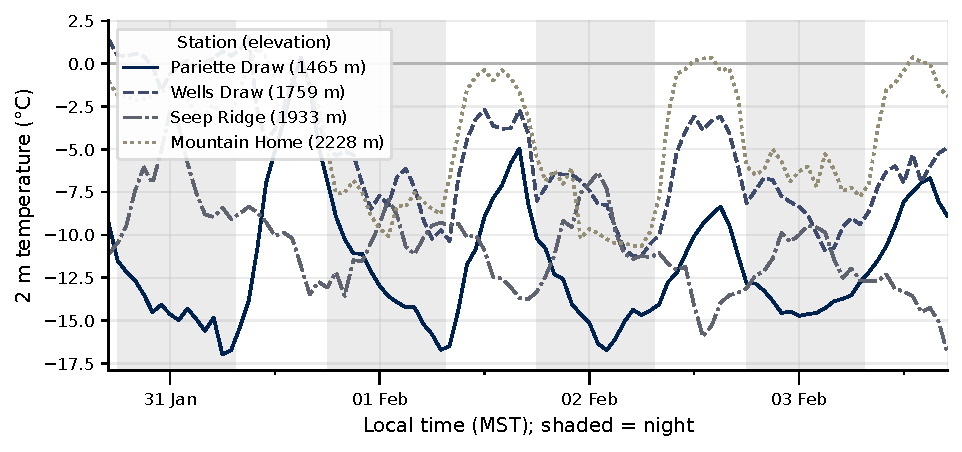
\includegraphics[width=\textwidth]{figures/obs_temp_timeseries_feb0102.pdf}
\caption{Observed 2 m-temperature evolution at four elevation-spanning Uinta Basin stations from 31 January through 3 February 2013.
Shading indicates approximate local night.
The sites establish a recurring spatial surface-temperature pattern but do not constitute a colocated vertical profile.}
\label{fig:v3-observed}
\end{figure}

\subsection{Common-Pipeline Contrasts at a Glance}
\label{sec:v3-effects-panel}

Figure~\ref{fig:v3-effects} places every controlled contrast evaluated with the frozen station/common-AGL pipeline on the same six metric axes before the individual result threads are interpreted.
It includes the two driving-product contrasts, the PBL/surface-layer and slope-radiation treatments, the three feedback contrasts across two terrain regimes, and the paired interaction.
The display adds no new computation; every dot and whisker is a committed summary value, and each row retains the differencing direction named in its label.
The driving-product response is the largest repeated separation in temperature, fixed-layer stability, and transport wind.
The PBL/surface-layer treatment is smaller but visibly distinct on several metrics, while the station-sample slope-radiation response, feedback responses, and interaction remain near zero at the driving-product scale.
The pressure and wind-error panels also prevent a single skill ranking: their signs and relative magnitudes do not reproduce the temperature and fixed-layer ordering.
The panel is a response hierarchy on one sample, not an omnibus judgment about which configuration is best.

\begin{figure}[H]
\centering
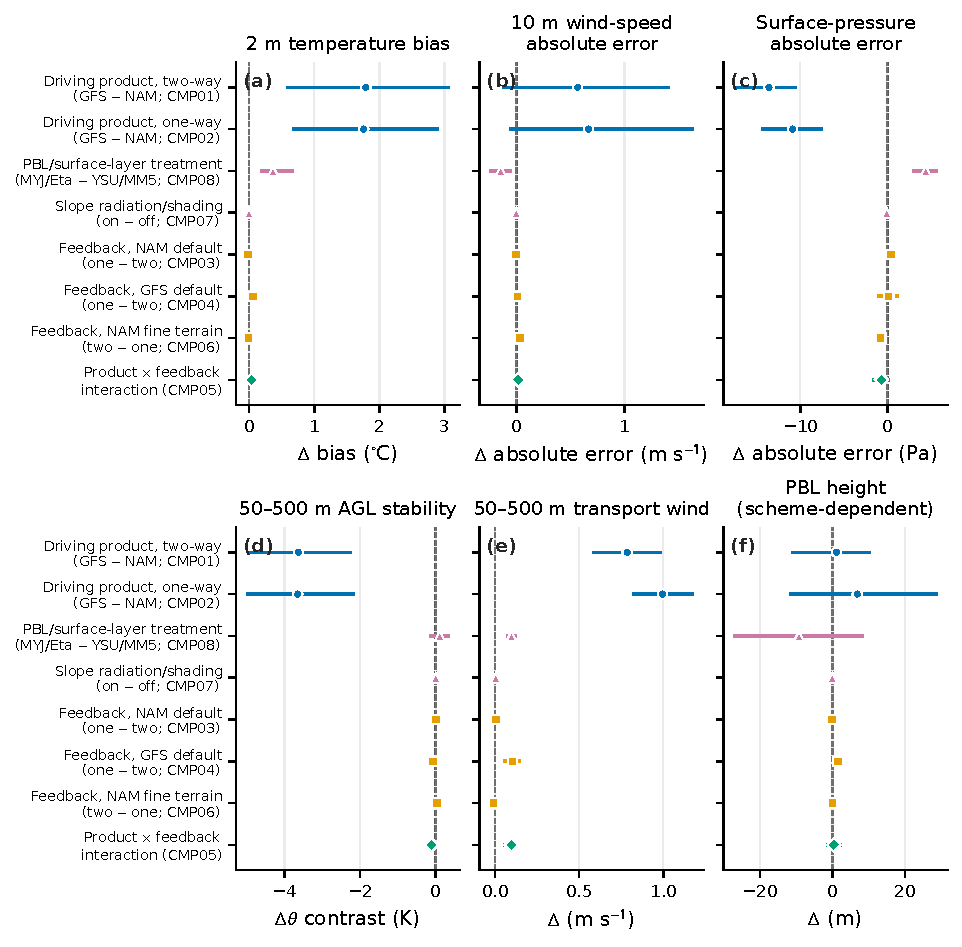
\includegraphics[width=\textwidth]{figures-draft/fig_common_pipeline_effects.pdf}
\caption{Common-pipeline contrast overview from the committed pair and interaction summaries: mean five-hour effects (markers) and descriptive two-hour circular block-sensitivity intervals (whiskers) for six metrics.
Blue circles are driving-product contrasts, purple triangles process treatments, orange squares feedback contrasts, and the green diamond the paired interaction; marker shape duplicates the color coding.
Rows retain their registered orientations: CMP03/CMP04 are one-way minus two-way, while CMP06 is two-way minus one-way.
The intervals are sensitivity descriptions of five dependent hourly medians, not confidence intervals.
Working figure drawn from committed data (\texttt{verification/scripts/plot\_common\_pipeline\_effects.py}); not yet registered or promoted.}
\label{fig:v3-effects}
\end{figure}

\subsection{Driving-Product Response in the Common Lower Layer}

The common-AGL diagnostics separated the driving products under both feedback settings (Figure~\ref{fig:v3-retention}).
GFS minus NAM reduced 50--500 m potential-temperature stability by 3.63 K under two-way feedback and 3.65 K under one-way feedback (Table~\ref{tab:v3-effects}).
The five hourly spatial-median differences ranged from -5.58 to -1.13 K and from -5.36 to -0.90 K, respectively.
All ten product-by-hour stability contrasts therefore retained the same sign.
GFS minus NAM increased fixed-layer transport wind by 0.79 m s$^{-1}$ under two-way feedback and 0.99 m s$^{-1}$ under one-way feedback.
The hourly differences ranged from +0.37 to +1.18 m s$^{-1}$ and from +0.61 to +1.50 m s$^{-1}$, with the same sign in every hour.
Native PBL-height differences changed sign within both feedback modes and did not reproduce the stability and wind separation.

\begin{figure}[H]
\centering
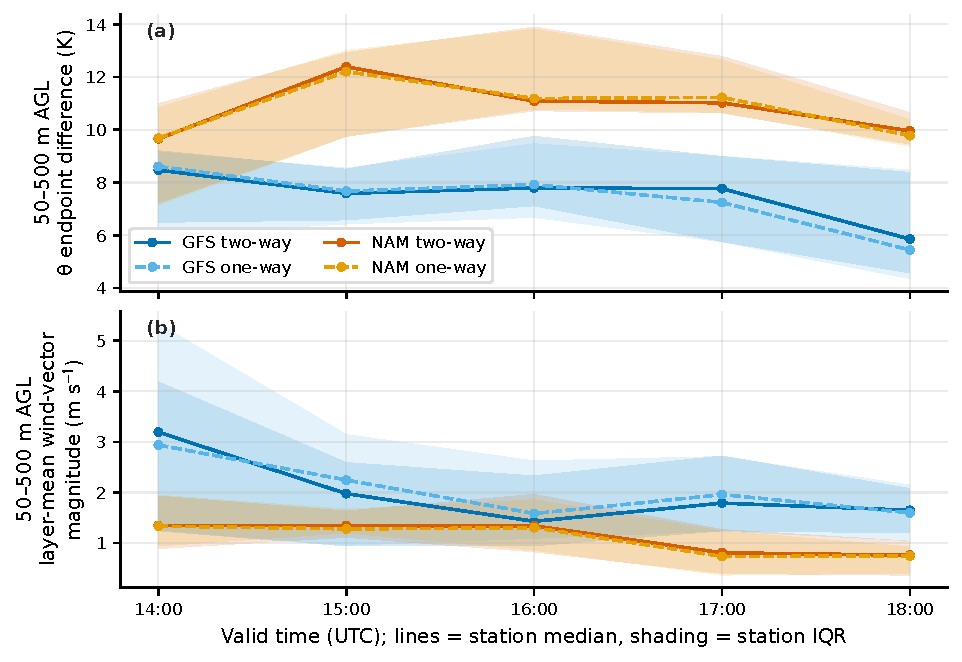
\includegraphics[width=\textwidth]{figures/wrf_retention_ventilation_d02_14to18.pdf}
\caption{Station-column medians and interquartile ranges for 50--500 m AGL potential-temperature stability, fixed-layer transport wind, and native WRF PBL height over the matched window.
Solid lines denote two-way feedback and dashed lines denote one-way feedback.
The lower-layer GFS--NAM separation recurs under both feedback modes, while PBL height is retained as a scheme-dependent companion rather than an observed layer depth.}
\label{fig:v3-retention}
\end{figure}

\begin{table}[H]
\caption{Paired effects for the default-terrain driving-product/feedback matrix, averaged over the five hourly spatial medians.
Positive temperature values indicate a warmer model-minus-observation bias, positive stability values indicate a more stable fixed layer, and positive transport-wind values indicate a larger layer-mean wind.
The effects are deterministic descriptive contrasts rather than inferential estimates.}
\label{tab:v3-effects}
\centering
\begin{tabular}{lrrr}
\toprule
Effect & $\Delta$T2 bias ($^{\circ}$C) & $\Delta S_{50:500}$ (K) & $\Delta U_{50:500}$ (m s$^{-1}$) \\
\midrule
GFS $-$ NAM, two-way & +1.79 & -3.63 & +0.79 \\
GFS $-$ NAM, one-way & +1.76 & -3.65 & +0.99 \\
GFS one-way $-$ two-way & +0.07 & -0.07 & +0.10 \\
NAM one-way $-$ two-way & -0.01 & +0.00 & +0.01 \\
Feedback interaction & +0.04 & -0.10 & +0.10 \\
\bottomrule
\end{tabular}
\end{table}

\subsection{Surface Corroboration and Metric-Dependent Skill}
\label{sec:v3-surface}

The paired surface-temperature result had the same product ordering as the layer diagnostics.
Mean hourly station-median 2 m-temperature biases were +2.09 and +2.51~$^{\circ}$C for the GFS members, against +0.40 and +0.60~$^{\circ}$C for the matched NAM members.
After pairing by station and hour, GFS minus NAM increased the temperature-bias contrast by +1.79~$^{\circ}$C under two-way feedback and +1.76~$^{\circ}$C under one-way feedback, and the corresponding absolute-error differences were +1.41 and +1.50~$^{\circ}$C (Table~\ref{tab:v3-effects}).
GFS minus NAM also increased 10 m-wind bias by +0.91 and +0.96 m s$^{-1}$, although the hourly difference in absolute wind error changed sign.
Surface pressure ordered the products in the opposite direction.
GFS minus NAM changed the paired surface-pressure absolute error by -13.6 Pa under two-way feedback and -10.9 Pa under one-way feedback, negative in all five hours, while all four members retained a positive mean pressure bias between +43 and +56 Pa on the nine-station sample.
These pressure differences are small in absolute terms, but their consistent sign shows that the surface metrics do not agree on a product ranking.
Aggregate surface skill is therefore metric-dependent for these simulations, and it cannot by itself establish which member supplies the more credible lower layer.

The two-site potential-temperature index provides the only direct observation-model comparison of lower-layer structure in this study.
Under two-way feedback, the GFS-driven member had a smaller Mountain Home-minus-Pariette Draw contrast than the matched NAM-driven member in every retained hour.
The observed spatial contrast ranged from 12.63 to 20.21 K, the NAM member from 16.44 to 18.07 K, and the GFS member from 7.35 to 11.74 K.
These two-site values combine elevation, horizontal distance, site exposure, and local surface energy balance, and they are not interpreted as free-air inversion depths.

\rewritegate{The existing bulk-theta render is withheld because its 8 K line came from a non-equivalent crest-relative sounding diagnostic.
On CHPC, regenerate the figure from the frozen real-observation cache with the updated line-free script, update hashes in both manifests, inspect the output, and re-promote it before restoring the figure here.}

\subsection{Spatial and Vertical Scope of the Driving-Product Response}
\label{sec:v3-spatial}

\diagnosticnote{Gate executed with a negative outcome.
The ANA-19 spatial-coherence analysis ran with predeclared criteria (job 13948410; ledger row C30): the shallow-confinement and fixed-column-consistency criteria passed at all ten pair-hours, but the floor sign-coherence criterion failed at 14:00--15:00 UTC, so the predeclared conjunction fails and no spatial figure is promoted.
The single figure retained below is a registered diagnostic candidate that displays the failed criterion directly; all numbers come from the committed summary tables, none from the image.}

The executed analysis quantifies the visual lead.
Over the registered evaluation footprint, the cell-area-weighted mean GFS-minus-NAM 2 m potential-temperature difference is positive at every retained hour under both feedback modes, growing from +0.89--+1.16 K at 14:00--15:00 UTC to +2.00--+2.74 K at 16:00--18:00 UTC (Figure~\ref{fig:v3-drivemaps}).
The footprint fraction sharing the median sign is 0.64--0.67 in the first two retained hours --- below the predeclared two-thirds threshold, which is why the gate fails --- and 0.84--0.93 at 16:00--18:00 UTC.
Vertical confinement passes at every pair-hour: the footprint mean of the absolute potential-temperature difference averaged over 50--500 m AGL exceeds the same quantity for 1500--2000 m AGL by factors of 1.45 to 3.12, and the ratio grows through the window.
The footprint-mean 50--500 m stability difference is negative at every pair-hour, from -3.04 to -4.33 K, matching the fixed-column result (C17), and the 1500--2000 m layer-mean difference itself turns weakly negative (-0.16 to -0.42 K) in the last two hours while the shallow layer stays strongly positive.
Because the predeclared floor-coherence criterion failed at the first two retained hours, Main C3 stays empty for this window; the committed summaries nevertheless document mean-sign coherence and shallow confinement explicitly, and the failure margin (0.001--0.025 below threshold) is recorded rather than argued away.

\begin{figure}[H]
\centering
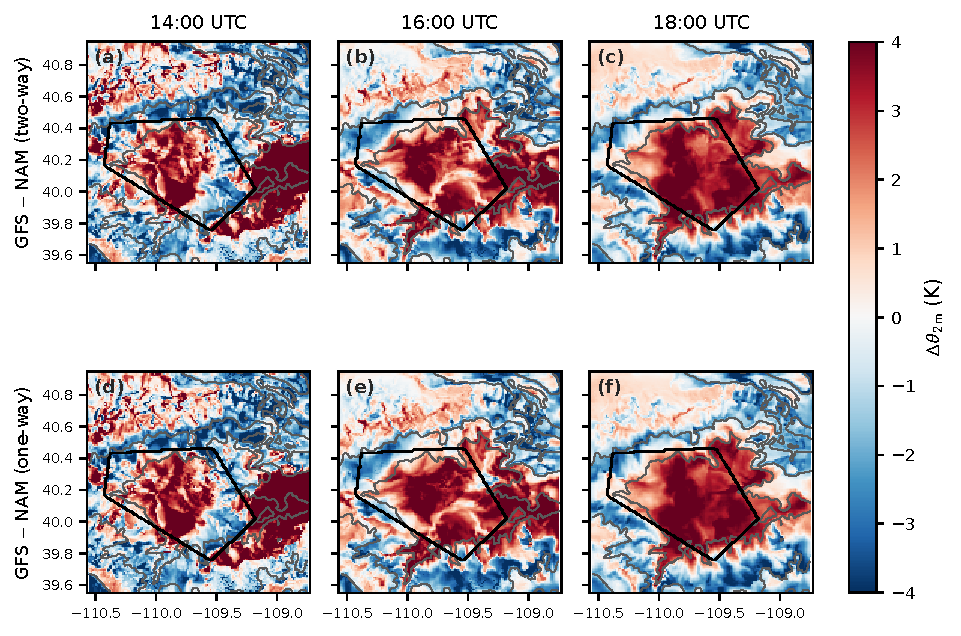
\includegraphics[width=\textwidth]{verification/figures/candidates/wrf_spatial_theta2m_diff_d02.pdf}
\caption{GFS-minus-NAM 2 m potential-temperature difference at the fixed display hours (14:00, 16:00, 18:00 UTC) under two-way (top, X6$-$X5) and one-way (bottom, X10$-$X3) feedback, with the registered evaluation footprint outlined in black and the 1700/2200 m terrain contours in gray.
Registered diagnostic candidate from the executed ANA-19 analysis (job 13948410); not promoted because the predeclared floor-coherence criterion failed at 14:00--15:00 UTC (C30).}
\label{fig:v3-drivemaps}
\end{figure}

\subsection{Footprint Heat Deficit: A Weaker State without Faster Loss}
\label{sec:v3-heatdeficit}

Under the primary definition, the footprint-mean heat deficit of the GFS members rose from 2.68 to 3.00 MJ m$^{-2}$ (two-way) and from 2.66 to 2.95 MJ m$^{-2}$ (one-way) between 14:00 and 18:00 UTC, while the matched NAM members rose from 4.18 to 4.33 and from 4.19 to 4.32 MJ m$^{-2}$ (Table~\ref{tab:v3-heatdeficit} and Figure~\ref{fig:v3-heatdeficit-traj}).
The paired GFS-minus-NAM differences averaged -1.23 MJ m$^{-2}$ under two-way feedback and -1.25 MJ m$^{-2}$ under one-way feedback.
All 70 retained pair-hour-definition differences were negative, spanning -1.80 to -0.70 MJ m$^{-2}$, so the weaker-state criterion passed in all 14 pair-definition combinations.
The faster-loss criterion required an actual GFS decrease that was also larger than the matched NAM change.
Instead, heat deficit increased in every member, by +0.32 and +0.30 MJ m$^{-2}$ for GFS and by +0.15 and +0.13 MJ m$^{-2}$ for NAM under two-way and one-way feedback.
The difference in change was +0.17 MJ m$^{-2}$ under both feedback modes for the primary definition and spanned -0.07 to +0.32 MJ m$^{-2}$ across definitions, without a consistent sign.
The faster-loss criterion therefore failed in all 14 pair-definition combinations.
The GFS-minus-NAM separation consequently narrowed slightly over the window, from -1.50 to -1.33 MJ m$^{-2}$ under two-way feedback and from -1.53 to -1.36 MJ m$^{-2}$ under one-way feedback.
The footprint result shows a consistently weaker simulated pool in the GFS members at every retained hour, not a divergence in its evolution.

\begin{figure}[H]
\centering
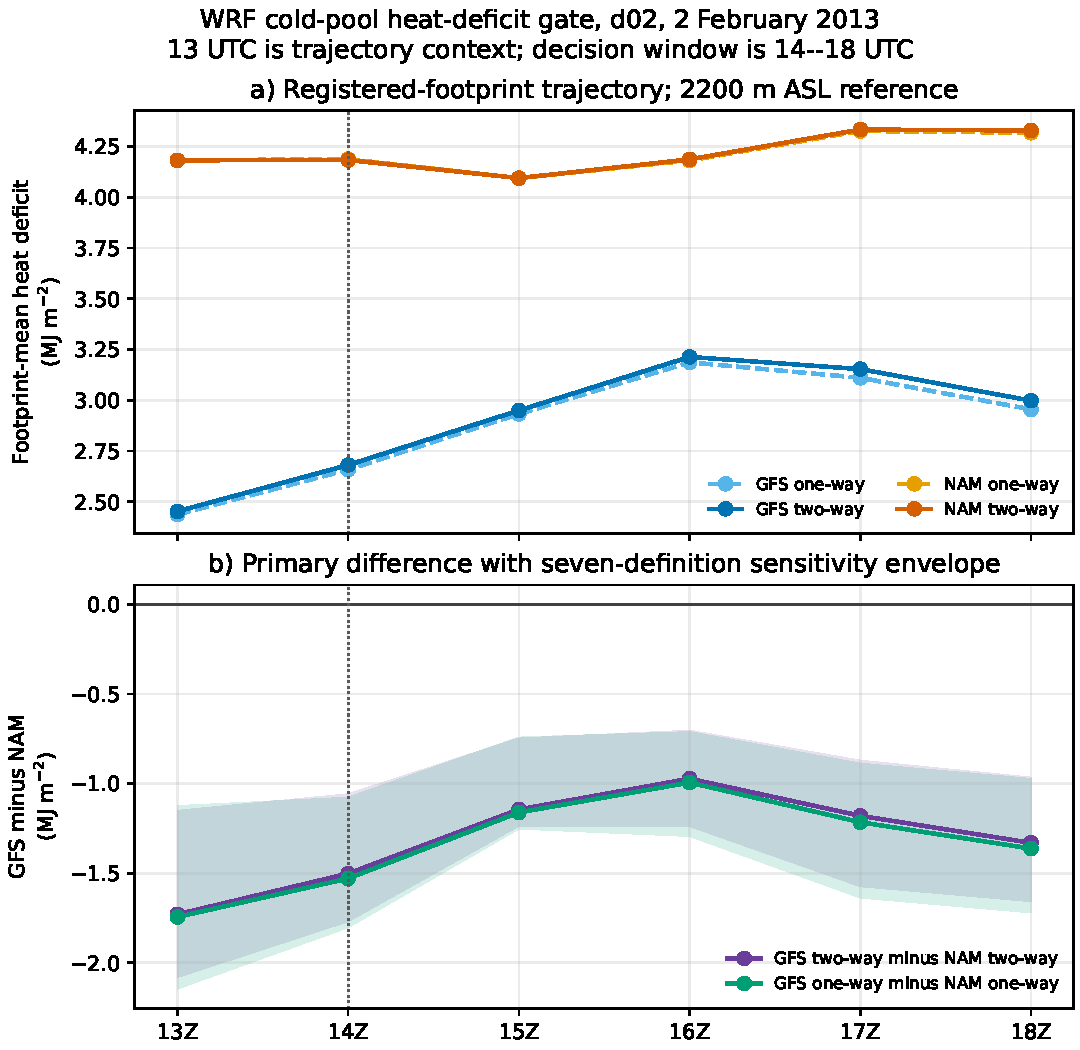
\includegraphics[width=0.9\textwidth]{verification/figures/candidates/wrf_heat_deficit_d02_13to18.pdf}
\caption{Footprint-mean heat-deficit trajectories for the four default-terrain matrix members from 13:00 to 18:00 UTC under the primary footprint definition, with the seven-definition sensitivity envelopes for the two GFS-minus-NAM pairs.
Registered candidate figure, visually inspected; the plotted values are the committed trajectory and sensitivity tables that also support Table~\ref{tab:v3-heatdeficit}.
The 13:00 UTC values are trajectory context only; all criteria use 14:00--18:00 UTC.}
\label{fig:v3-heatdeficit-traj}
\end{figure}

\begin{table}[H]
\caption{Footprint-integrated heat-deficit contrasts over the 14:00--18:00 UTC decision window.
The primary definition uses the combined station-and-waypoint hull with a 2200 m crest (4965 cells, 5277 km$^{2}$); envelopes span all seven footprint definitions.
The values are deterministic descriptive contrasts in MJ m$^{-2}$.}
\label{tab:v3-heatdeficit}
\centering
\begin{tabular}{lrr}
\toprule
GFS $-$ NAM quantity & Two-way pair & One-way pair \\
\midrule
Mean difference (primary) & -1.23 & -1.25 \\
Hourly range (primary) & -1.50 to -0.97 & -1.53 to -0.99 \\
Hourly envelope (seven definitions) & -1.77 to -0.70 & -1.80 to -0.71 \\
GFS change, 14:00--18:00 UTC & +0.32 & +0.30 \\
NAM change, 14:00--18:00 UTC & +0.15 & +0.13 \\
Difference in change (primary) & +0.17 & +0.17 \\
Weaker-state criterion passed & 7/7 & 7/7 \\
Faster-loss criterion passed & 0/7 & 0/7 \\
\bottomrule
\end{tabular}
\end{table}

\subsection{Process Treatments on the Fine-Terrain Branch}
\label{sec:v3-process}

\diagnosticnote{Screen executed (jobs 13948412 and 13948378; ledger rows C31 and C32).
CMP08 produced the strongest coherent non-driving-product response on the frozen station pipeline and is the sole remaining Main C6 candidate.
CMP07 failed its predeclared shortwave criterion for the measurement-limited reason recorded below.
The archived run summaries for X1 and X2 still expose no source-code commit, a standing provenance caveat.}

The scheme pair (CMP08, X2$-$X1) changes only the boundary-layer and surface-layer schemes, MYJ/Eta against YSU/MM5, while holding the fine terrain and slope-aware radiation configuration fixed.
MYJ/Eta warms the 2 m-temperature bias by +0.37~$^{\circ}$C in all five hours, reduces the 10 m-wind absolute error by 0.145 m s$^{-1}$ in all five hours, raises the surface-pressure bias by +6.3 Pa in all five hours, and increases the fixed-layer transport wind by +0.098 m s$^{-1}$ in all five hours with a block interval of +0.069 to +0.126 m s$^{-1}$ (Table~\ref{tab:v3-process}; C32).
The stability response is mixed (+0.11 K, three positive hours of five, interval spanning zero), and the 9.2 m PBL-height decrease is scheme-defined and carries no common structural meaning across schemes.
The response is smaller than the driving-product contrast on every shared lower-layer metric but larger than the feedback responses; the ratio depends strongly on the metric and should not be reduced to a single order-of-magnitude statement.
Temperature error worsens while wind error improves, providing another within-archive example of metric-dependent skill rather than a scheme ranking.
The exploratory 16:00 UTC map and section are not retained: at manuscript scale they are unreadable, and no spatial criterion has been predeclared for them.
Editorial review must still decide whether the confirmed station contrast belongs in the main text or supplement.

\begin{table}[H]
\caption{Executed process-pair station contrasts on the frozen pipeline (14:00--18:00 UTC; job 13948378).
Values are means of five hourly spatial medians; sign counts are positive/negative hours with exact zeros omitted; intervals are the descriptive two-hour circular block resample, not confidence intervals.
PBL height is scheme-defined across CMP08 and is retained only with that caveat.}
\label{tab:v3-process}
\centering
\footnotesize
\begin{tabular}{lrrrr}
\toprule
Metric & \multicolumn{2}{c}{CMP07 (X1 $-$ X0)} & \multicolumn{2}{c}{CMP08 (X2 $-$ X1)} \\
 & Mean & Signs & Mean & Signs \\
\midrule
T2 bias ($^{\circ}$C) & +0.001 & 3/1 & +0.37 & 5/0 \\
10 m wind absolute error (m s$^{-1}$) & +0.001 & 2/2 & -0.145 & 0/5 \\
Surface-pressure bias (Pa) & -0.12 & 0/4 & +6.3 & 5/0 \\
Stability $S_{50:500}$ (K) & +0.004 & 3/1 & +0.11 & 3/2 \\
Transport wind $U_{50:500}$ (m s$^{-1}$) & +0.006 & 4/0 & +0.098 & 5/0 \\
PBL height (m) & +0.01 & 3/1 & -9.2 & 2/3 \\
\bottomrule
\end{tabular}
\end{table}

The slope-aware radiation pair (CMP07, X1$-$X0) enables slope-aware radiation and topographic shading with the archived 25 km shadow length; those are the only configuration differences, and the members are bitwise identical at initialization.
The archived SWDOWN diagnostic remains a flat-plane value and changes by no more than 0.27 W m$^{-2}$ in the aspect contrast, while no surface heat fluxes were archived, so the predeclared shortwave criterion fails on a diagnostic that cannot express the applied treatment (C31).
The surface nevertheless responds where the treatment acts: south-facing steep cells warm relative to north-facing steep cells by +1.08 to +2.23 K in skin temperature and +0.16 to +0.90 K in 2 m potential temperature at every post-sunrise hour (Figure~\ref{fig:v3-radiationpanel}).
The station-column response is essentially null (stability +0.004 K, transport wind +0.006 m s$^{-1}$, and temperature bias +0.001~$^{\circ}$C), because the frozen stations sample the floor rather than the affected slopes.
The registered aspect panel is therefore retained as the single diagnostic figure for CMP07; the redundant sunrise/late-morning maps and adaptively scaled heat-deficit panels remain reproducible in the figure harvest but are removed from the manuscript.

\begin{figure}[H]
\centering
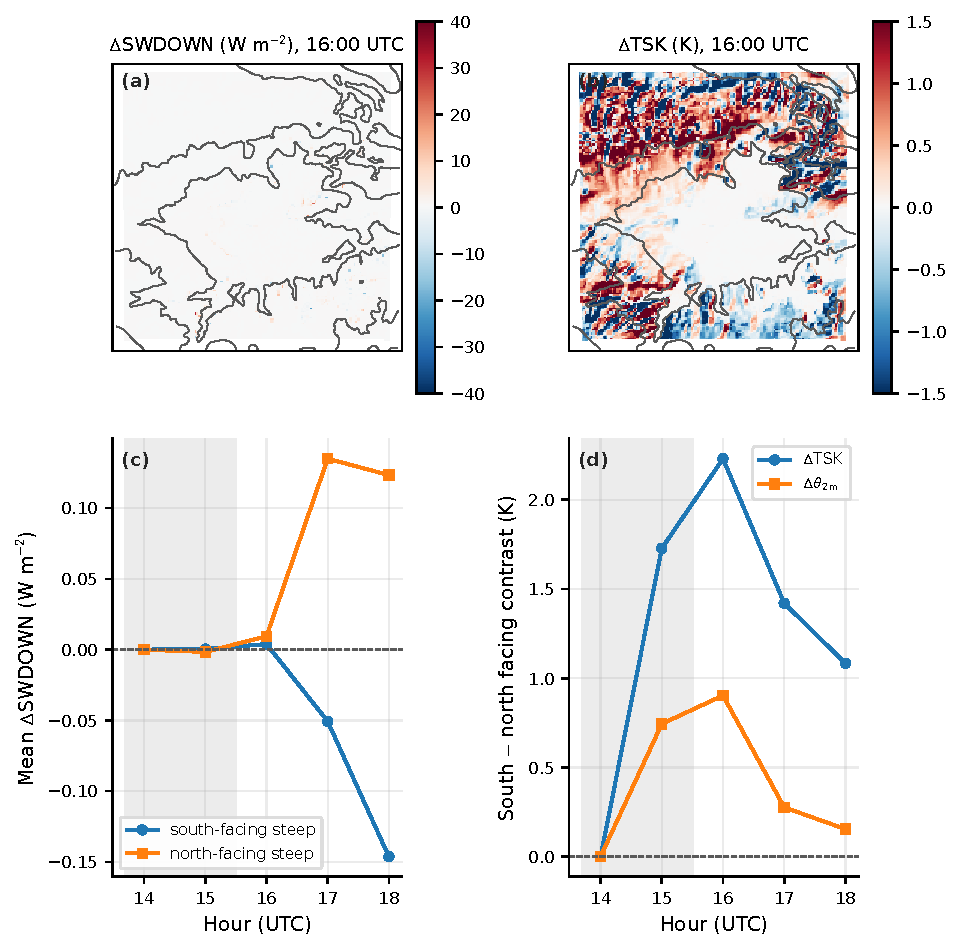
\includegraphics[width=\textwidth]{verification/figures/candidates/wrf_radiation_response_cmp07_d02.pdf}
\caption{Registered diagnostic panel for the executed CMP07 screen (ANA-18, job 13948412): (a) the unresponsive flat-plane $\Delta$SWDOWN field and (b) the aspect-organized $\Delta$TSK field at 16:00 UTC; (c) mean $\Delta$SWDOWN on south- and north-facing steep cells by hour; (d) the south-minus-north facing contrast in skin temperature and 2 m potential temperature.
Shading marks the pre-/near-sunrise hours excluded from the decision criteria.
The predeclared shortwave criterion failed for the recorded measurement-limited reason; the skin-temperature response is a committed diagnostic, not a gate-passed claim (C31).}
\label{fig:v3-radiationpanel}
\end{figure}

\subsection{Nest-Feedback Robustness across Two Terrain Regimes}
\label{sec:v3-feedback}

\subsubsection{Default-terrain bounds}
The within-product feedback responses were much smaller than the GFS-minus-NAM contrasts, but they were not identical between products (Table~\ref{tab:v3-effects}).
For NAM, one-way minus two-way averaged +0.002 K for stability and +0.006 m s$^{-1}$ for transport wind, and the hourly effects changed sign within -0.042 to +0.088 K and -0.035 to +0.033 m s$^{-1}$.
For GFS, one-way minus two-way averaged -0.066 K for stability and +0.104 m s$^{-1}$ for transport wind.
The GFS stability effect ranged from -0.198 to +0.067 K and was negative in four of five hours, while the transport-wind effect ranged from +0.025 to +0.197 m s$^{-1}$ and was positive in all five hours.
The paired feedback interaction averaged -0.103 K for stability and +0.097 m s$^{-1}$ for transport wind, with the wind component positive in all five hours.
The 2 m-temperature-bias interaction was +0.041~$^{\circ}$C, and the PBL-height interaction changed sign from hour to hour.
These values bound the response of the present configuration and sample; they do not establish general equivalence between feedback modes.

\subsubsection{Fine-terrain replication (CMP06)}
\label{sec:v3-cmp06}

The fine-terrain control pair, X9 minus X0, isolates the same feedback flag as the default-terrain contrasts but at the 3-arc-second static terrain of the control configuration.
Recomputed on exactly the default-terrain matrix's matched surface and common-AGL definitions (Section~\ref{sec:v3-expanded-diagnostics}), every fine-terrain feedback effect is again one to two orders of magnitude smaller than the matched driving-product contrast (Table~\ref{tab:v3-cmp06}).
Two-way minus one-way stability averaged +0.04 K (hourly range -0.09 to +0.14 K, positive in four of five hours), transport wind -0.01 m s$^{-1}$ (range -0.07 to +0.03 m s$^{-1}$, mixed signs), and 2 m-temperature bias -0.004~$^{\circ}$C (range -0.09 to +0.04~$^{\circ}$C, mixed signs).
The block-sensitivity intervals for stability, transport wind, PBL height, and temperature bias all span zero.
The two metrics with consistent hourly sign are small: 10 m-wind absolute error increased by +0.03 m s$^{-1}$ in all five hours, and surface pressure decreased by -0.77 Pa in bias and absolute error in all five hours on the nine-station sample.
For comparison at the same terrain and physics, the CMP01 and CMP02 driving-product contrasts move stability by more than 3.6 K and transport wind by 0.8 to 1.0 m s$^{-1}$.
The bounded-feedback conclusion therefore survives the change of terrain regime.
This recomputation passed its predeclared gate (the ANA-20 falsifier --- a fine-terrain feedback effect approaching the driving-product magnitude --- did not occur) and is recorded as ledger row C28; no figure is promoted because the quantitative table carries the result without a redundant near-null map.

\begin{table}[H]
\caption{Fine-terrain feedback contrast CMP06 (X9 minus X0, \emph{two-way minus one-way}, the authoritative orientation of the comparison inventory and the reverse of the feedback rows in Table~\ref{tab:v3-effects}).
Values are means of five hourly spatial medians from the committed recomputation (job 13948333), with hourly ranges, sign counts, and descriptive two-hour block-sensitivity intervals.
Sensitivity intervals are not confidence intervals.}
\label{tab:v3-cmp06}
\centering
\footnotesize
\begin{tabular}{lrrrr}
\toprule
Metric & Mean & Hourly range & Signs ($+$/$-$) & Sens.\ interval \\
\midrule
Stability $S_{50:500}$ (K) & +0.04 & -0.09 to +0.14 & 4/1 & -0.03 to +0.10 \\
Transport wind $U_{50:500}$ (m s$^{-1}$) & -0.01 & -0.07 to +0.03 & 3/2 & -0.03 to +0.01 \\
PBL height (m) & +0.05 & -0.67 to +0.78 & 3/2 & -0.38 to +0.47 \\
T2 bias ($^{\circ}$C) & -0.004 & -0.09 to +0.04 & 3/2 & -0.05 to +0.03 \\
T2 absolute error ($^{\circ}$C) & -0.006 & -0.06 to +0.05 & 2/3 & -0.04 to +0.03 \\
10 m wind bias (m s$^{-1}$) & +0.02 & -0.01 to +0.06 & 4/1 & +0.01 to +0.04 \\
10 m wind absolute error (m s$^{-1}$) & +0.03 & +0.001 to +0.06 & 5/0 & +0.01 to +0.06 \\
Surface-pressure bias (Pa) & -0.77 & -1.23 to -0.35 & 0/5 & -1.06 to -0.50 \\
Surface-pressure absolute error (Pa) & -0.77 & -1.23 to -0.42 & 0/5 & -1.01 to -0.59 \\
\bottomrule
\end{tabular}
\end{table}

\subsection{Terrain-Source Brackets (CMP09--CMP11)}
\label{sec:v3-terrain}

\diagnosticnote{Gate executed: CMP09 failed its predeclared criteria, and the X4 lineage check passed, closing that standing caveat (job 13948411; \texttt{verification/data/terrain\_response\_criteria.csv}; ledger row C29).
No terrain slot is promoted; the quantitative values below are committed descriptive diagnostics, not gate-passed claims.}

The archive brackets the static terrain source on an otherwise identical NAM one-way configuration: default minus fine (CMP09, X3$-$X0), default minus coarse (CMP10, X3$-$X4), and fine minus coarse (CMP11, X0$-$X4).
The executed analysis first resolves identity: the archived X4 \texttt{namelist.input} hashes byte-identically to the X0/X3 namelist, and its terrain is far smoother than the default member's, so the coarse-terrain member is confirmed as the same configuration family with only the static source changed (C29), and CMP10/CMP11 are controlled comparisons.
The fine bracket itself is small on this grid: the X3-minus-X0 terrain difference has a root-mean-square of only 7.9 m (range -55 to +60 m), and its 2 m response is correspondingly small, with elevation-band means of 0.07--0.27 K (Figure~\ref{fig:v3-terrainpanel}).
The response is slope-organized --- the slopes-band mean exceeds the floor band by factors of 1.7--2.4 at every hour, passing the first predeclared criterion --- but its area-weighted correlation with the terrain difference stays below the predeclared 0.3 magnitude at 14:00--16:00 UTC (reaching 0.34--0.36 only late in the window), so the CMP09 gate fails and Main C5 stays empty for this window.
The coarse brackets are an order of magnitude larger (terrain RMS 91.9 and 93.1 m, ranges to -462/+487 m) and their committed diagnostics are correspondingly stronger: slopes-band responses of 1.2--1.5 K, terrain correlations of 0.50--0.67 at every hour, and station-sample mean responses up to +0.61 K.
No gate was predeclared for the coarse brackets, so those values carry no claim; declaring and testing one is now unblocked by the lineage closure.
Per-station model-minus-station elevations for all three members are committed (\texttt{verification/data/terrain\_station\_elevation.csv}), making the pressure-artifact mechanism of Section~\ref{sec:v3-disc-terrain} directly checkable.
The registered CMP09 panel is retained to document the failed criteria and their margins; the engine map/section gallery and threshold-sensitive heat-deficit prototype remain reproducible outside the manuscript because no gate-passed claim requires them.

\begin{figure}[H]
\centering
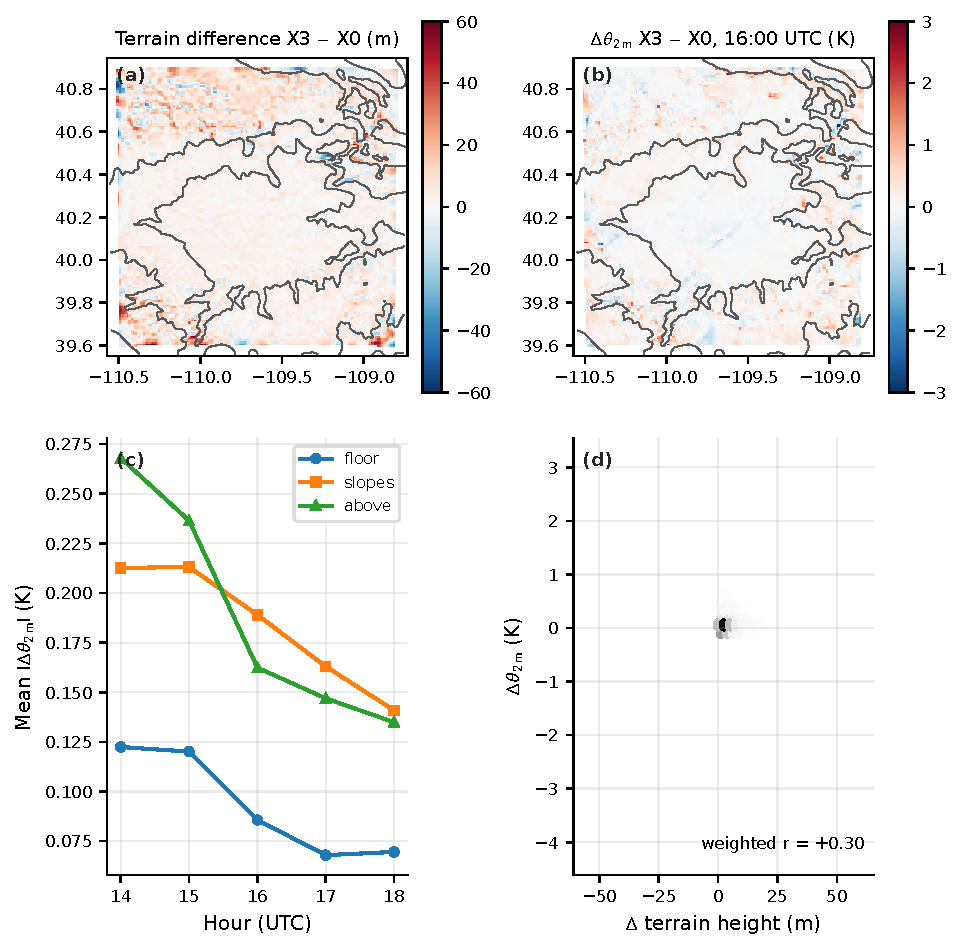
\includegraphics[width=\textwidth]{verification/figures/candidates/wrf_terrain_response_cmp09_d02.pdf}
\caption{Registered diagnostic panel for the executed CMP09 analysis (ANA-17, job 13948411): (a) the X3$-$X0 terrain difference; (b) the 2 m potential-temperature response at the fixed 16:00 UTC display hour; (c) elevation-band means of the absolute response by hour; (d) the response-versus-terrain-difference density with the area-weighted correlation.
The slope-organization criterion passed and the terrain-correlation criterion failed, so no promotion follows (gate review; C29 covers the lineage closure only).}
\label{fig:v3-terrainpanel}
\end{figure}

\section{Discussion}

\subsection{A Product-Level Difference, Not a Universal Product Ranking}

The principal result is a replicated product-level separation.
The GFS-driven members are warmer at the evaluated surface sites, less stable across the fixed 50--500 m layer, faster in the fixed-layer transport metric, and lower in footprint-integrated heat deficit than the NAM-driven members under both feedback settings.
Replication across the feedback flag makes this ordering insensitive to that one configuration choice within the default-terrain matrix.
It does not establish that NAM is generally superior, and the opposite ordering of the surface-pressure errors shows that even the present surface evaluation does not support a single-metric ranking.
The driving-product treatment combines the 12:00 UTC initial atmosphere with boundary updates through 18:00 UTC.
A direct comparison of each product with an independent profile at initialization would test inherited lower-tropospheric error, and an experiment that holds either the initial or boundary state fixed would be needed to apportion the subsequent response.
Until those tests exist, ``driving-product response'' is more accurate than ``initial-condition effect.''

\subsection{What the Difference Means for an Air-Quality Model}

The GFS members supplied a less stable, faster-moving, and lower-heat-deficit lower layer over the evaluated columns and footprint.
That combination is consistent with a meteorological state more favorable to dilution than the matched NAM state.
The distinction is relevant because a chemistry calculation is constrained by the mixing volume and transport in its meteorological input; changing chemistry alone cannot test whether a missing shallow accumulation layer caused a concentration error.
The footprint heat deficit extends the fixed-column result to an area integral of the simulated pool: the GFS members carried 0.70 to 1.80 MJ m$^{-2}$ less deficit at every retained hour under every footprint definition.
However, the transport-wind metric does not measure pollutant export, the heat-deficit footprint is not an observed volume, and no chemical species were simulated.
This boundary is important in the Uinta Basin literature.
Inventory changes, snow and cloud treatment, deposition, chemical mechanisms, and meteorological confinement have all produced substantial responses in designs that were often cumulative, bundled, or conditional on one meteorological platform \citep{Ahmadov2015-zm,Neemann2015-ws,Matichuk2017-bq}.
An improved meteorological state need not yield improved ozone if another component changes or compensates.
The present result therefore identifies a meteorological precondition for attribution rather than assigning an ozone effect or ranking all sources of model error.

\subsection{A Predeclared Heat-Deficit Test and Its Negative Result}

The heat-deficit analysis carried two criteria that were fixed before any output was inspected.
The weaker-state criterion passed unanimously and extends the fixed-column stability result to an area-integrated measure of the simulated pool.
The faster-loss criterion failed unanimously because the heat deficit of every member increased through the morning window.
We report that outcome rather than relaxing the criterion after inspection.
The correct reading is a state offset that was already present at the first retained hour, not a demonstrated within-window divergence in pool evolution between the products.
A hypothesis that the GFS members progressively deplete the simulated pool is not supported on this window.
Testing differential heat-deficit loss at all would require a longer matched integration through at least one diurnal cycle, with the same predeclared footprint and criteria.

\subsection{Where the Driving-Product Response May Live}
\label{sec:v3-disc-spatial}

The executed ANA-19 analysis converts the spatial hypothesis into a split verdict.
The confinement half is now demonstrated in committed summaries: the response is concentrated in the 50--500 m layer over the footprint at every pair-hour, with confinement ratios growing from about 1.5 to 3.1 through the window, and the footprint-mean signs match the fixed-column result throughout (C30).
The coherence half failed its predeclared bar: at 14:00--15:00 UTC roughly a third of the footprint area carries the opposite 2 m sign, so the gate's two-thirds criterion fails and no spatial figure is promoted, even though the same criterion passes strongly from 16:00 UTC onward.
The honest reading is that the driving-product response is real, shallow, and mean-coherent, but not yet spatially unanimous at the start of the retained window under this criterion; a future gate could predeclare a different bar, and this draft does not.
An experiment that swaps initial and boundary sources between the products remains the designed follow-up.

\subsection{Process Treatments as Bounded Questions}
\label{sec:v3-disc-process}

The two process pairs posed different kinds of questions, and the executed screen answered both.
The slope-radiation pair delivered a bounded, instructive outcome: the treatment acts exactly where its physics says it should --- an aspect-organized skin-temperature contrast of one to two kelvin on the sidewalls --- while remaining invisible to station means on the basin floor and to the archived flat-plane shortwave diagnostic (C31).
That is a measurement lesson as much as a physics result: evaluating slope-aware radiation in this archive requires skin-temperature or newly output slope-corrected flux fields, and any future CMP07 gate must be predeclared on instruments the archive can actually express.
The scheme pair delivered the coherent result the provisional C19 hinted at: consistently signed shifts across temperature, wind error, pressure, and transport wind (C32), smaller than the driving-product response on the core lower-layer metrics but by a ratio that varies substantially among metrics.
The honest framing remains a process-treatment comparison rather than a scheme skill contest, because PBL height is scheme-defined and only the MYJ member exposes \texttt{TKE\_PBL}.
The screen therefore selects CMP08 as the sole Main C6 candidate on coherence and information gain, with its main-versus-supplement disposition left to review.
Neither pair alters the paper's anchor result: for the temperature, stability, and transport-wind metrics that define that result, the repeated driving-product response remains larger than either process-treatment response.

\subsection{Nest Feedback as a Replicated Robustness Result}
\label{sec:v3-disc-feedback}

With the CMP06 recomputation (C28), the feedback question now has a consistent answer at two terrain regimes: within-product feedback effects are one to two orders of magnitude smaller than the driving-product contrast at default terrain and at the fine-terrain control, with sensitivity intervals that span zero for the primary lower-layer metrics in both regimes.
The only consistently signed fine-terrain feedback effects --- slightly larger absolute 10 m wind error and slightly lower surface pressure in the two-way member --- are small enough to carry no configuration recommendation on their own.
This is the appropriate role for the feedback lever in this study: a replicated robustness check that protects the driving-product conclusion, not a thesis.
The result is specific to this case, window, domain geometry, and diagnostic set, and it licenses no general claim about nest feedback in other regimes or seasons.

\subsection{Terrain as Geometry and Capacity, Not a Score Shortcut}
\label{sec:v3-disc-terrain}

The terrain bracket is scientifically attractive precisely because its aggregate scores are unremarkable: if terrain-source choice reorganizes the simulated pool along rims and tributaries without moving station means, then station-mean skill is the wrong instrument for terrain decisions in this basin.
The executed ANA-17 analysis sharpens that framing in both directions.
The fine bracket turns out to be physically small on this grid --- an 8 m root-mean-square terrain change producing a 0.1--0.3 K, slope-organized response --- and it failed the predeclared terrain-correlation criterion early in the window, so no terrain slot is filled from CMP09.
The coarse brackets are the opposite: an order of magnitude larger in both terrain change and response, strongly terrain-correlated at every hour, and now cleanly controlled because the X4 lineage check closed the archive-path caveat (C29).
The committed per-station elevation table makes the pressure-artifact mechanism concrete: the coarse member's near-zero mean pressure bias coexists with large station terrain displacement, a reminder that pressure agreement can be a terrain artifact rather than skill.
A coarse-bracket geometry gate is therefore the natural next predeclaration; until one passes, no terrain ranking of any kind is offered.

\subsection{Design Lessons from Confounded and Legacy Configurations}
\label{sec:v3-disc-design}

The apparent resolution ladder earns its place in the paper as a refusal.
Simultaneous confounds across X7, X0, and X8 (Table~\ref{tab:v3-confounds}) mean that any skill difference among them is unattributable, and presenting them as a resolution result would manufacture a conclusion the archive cannot support.
The same discipline applies to legacy nudged and SIP-era runs: they motivate design requirements --- matched initialization, single-lever differences, recorded as-run namelists, and provenance fingerprints --- but they cannot be ranked against the controlled family.
These negative design findings are inexpensive to state and materially useful to the next experiment, which is why they are retained in a paper otherwise built from positive controlled contrasts.

\subsection{Why the Common-AGL Result Leads the Paper}

This draft gives the common-AGL panel priority over both the surface scores and the two-site index.
The surface metrics disagree with one another: temperature favors NAM strongly, pressure favors GFS consistently but weakly, and the wind-error ordering depends on the error definition.
A single aggregate surface score would therefore conceal exactly the layer behavior the driving-product contrasts were designed to expose.
The two-site index is useful descriptive context and supplies a direct observation-model comparison of a floor-to-bench potential-temperature contrast, but its stations are horizontally separated, only its two-way product pair is shown, and it cannot validate a free-air inversion.
By contrast, the common-AGL calculation applies the same geometric layer, fixed columns, valid times, and aggregation to all four simulations and directly displays both axes of the default-terrain matrix.
Native PBL height is not a replacement for that calculation: its product contrasts changed sign, and its physical meaning depends on the boundary-layer scheme.
This behavior follows the broader lesson from data-assimilation and cold-pool studies that diagnosed PBL depth, nudging reach, and evaluation-grid structure must be disclosed rather than treated as interchangeable \citep{Tran2018-ax,Neemann2015-ws}.

\subsection{What d02 Measures and What It May Hide at d03}
\label{sec:v3-disc-domains}

The d02 choice is a coverage decision, not a finding that 1 km is the scientifically sufficient grid or that d02 is more accurate than d03.
It preserves the eleven-station floor-to-bench sample and the full registered footprint, whereas a d03-only station evaluation would retain only four interior columns and silently change the estimand.
That makes d02 the defensible domain for the claims reported here, but it does not establish that the contrast magnitudes transfer to the 333 m nest.

A d02 analysis can plausibly attenuate a response whose mechanism is localized to slopes, tributaries, drainage channels, or sharp terrain gradients.
That concern is most material for the terrain-source and slope-radiation treatments and may also matter for nest-feedback effects near terrain and nest boundaries.
Conversely, a detailed d03 pattern without a common footprint or independent observations can look more physically persuasive while providing a weaker evaluation.
The current evidence therefore cannot say that any simulation is undervalued on d02; it can only say that subkilometer response transfer remains untested.

The appropriate follow-up is a predeclared domain-transfer diagnostic rather than a claim that one nest is better.
For each selected controlled contrast, d02 should first be restricted to a boundary-buffered d03 interior, d03 should be conservatively aggregated to the same support, and the contrast-of-contrasts $[X_a-X_b]_{d03}-[X_a-X_b]_{d02}$ should be evaluated for sign, magnitude, and spatial organization.
A second leg should sample the same four interior stations from both domains, so that a domain change is not confounded with a station-sample change.
Those tests would determine whether the present response hierarchy survives at 333 m; they would still not constitute an independent grid-spacing experiment because the nests differ in support, terrain representation, and nested forcing.

\subsection{Limits That Determine the Next Experiment}

The five-hour window is the strongest limit.
It can show a coherent short-window separation but cannot establish multi-day retention, event buildup, or cold-pool breakup, and the heat-deficit trajectories cover the same five hours.
The two-hour spin-up exclusion has not been varied, and resampling five dependent hourly medians cannot create an inferential sample.
The observation network creates a second limit.
Four stations establish surface context and eleven fixed columns support matched comparisons, but neither set observes the modeled vertical layer, and small nearest-cell elevation errors do not remove exposure and representativeness error.
Independent in-basin vertical observations are required to evaluate inversion depth, layer stability, and the simulated heat deficit directly.
Observation provenance and the full model-configuration record must also be completed before submission, as marked by the rewrite gates in this draft.
All five evidence gates of the selected results architecture have now been executed with predeclared criteria (the complete decision record is the hybrid gate review): the fine-terrain feedback bound passed (Section~\ref{sec:v3-cmp06}); the heat-deficit maintenance leg, the spatial-coherence conjunction, and the fine-terrain-bracket geometry criteria failed and are reported as negatives with their margins; and the process screen selected the boundary-layer-scheme contrast as the sole remaining candidate slot, pending editorial review.
Failed gates were not relaxed after inspection, and any renewed spatial or terrain claim requires a freshly predeclared criterion rather than a rescue of a failed one.
Only after those steps should selected meteorological states be crossed with emissions and chemical mechanisms in a coupled attribution experiment.

\section{Conclusions}

Across the controlled archive for the 2 February 2013 Uinta Basin episode, the common-pipeline contrasts form an evidence-based response hierarchy rather than a run-number sequence.
The largest repeated five-hour response is the driving-data-product contrast in the four-run default-terrain matrix on the common d02 evaluation sample.
Relative to NAM, GFS is warmer at the evaluated surface sites, less stable from 50 to 500 m AGL, faster in the fixed-layer transport-wind metric, and 0.70 to 1.80 MJ m$^{-2}$ lower in footprint-integrated heat deficit at every retained hour, under both one-way and two-way nest feedback.
Surface-pressure errors order the products in the opposite direction, so aggregate surface skill alone would not identify these lower-layer differences.
A predeclared faster-loss criterion for the GFS heat deficit failed in all fourteen pair-definition combinations because the deficit increased in every member; the driving-product response is a state offset within this window, not a demonstrated difference in pool evolution.
The PBL/surface-layer treatment is the strongest coherent non-driving contrast on the same station pipeline, but it is smaller on the core lower-layer metrics and splits the surface-skill verdict by warming temperature bias while reducing wind error.
The within-product feedback responses are much smaller for all evaluated diagnostics, and a matched recomputation at the fine-terrain control pair reproduces that bound, with every fine-terrain feedback effect one to two orders of magnitude below the matched driving-product contrast and with sensitivity intervals spanning zero for the primary lower-layer metrics.
All five evidence gates of the selected results architecture were executed for this revision with predeclared criteria: beyond the passing feedback bound, the spatial analysis demonstrated shallow confinement while failing its floor-coherence bar at the first two retained hours, the terrain analysis closed the coarse-member lineage caveat while the fine bracket failed its correlation bar, and the process screen recorded a measurement-limited radiation outcome while selecting a coherent boundary-layer-scheme contrast --- warmer temperature bias, smaller wind error, stronger transport wind, all consistently signed --- as the one remaining candidate result.
Failed gates are reported as negatives with their margins; nothing was promoted, and the surrounding exploratory material sharpens the questions the next revision can answer without altering the present conclusions.
The result establishes a short-window difference in the meteorological state available to downstream chemistry; it does not identify the responsible product component, validate inversion depth, demonstrate event-scale persistence, calculate basin export, or predict ozone.
Because d02 was selected to retain the eleven-station network rather than validated against d03, the present hierarchy must not be assumed to hold unchanged on the 333 m interior nest.
The next discriminating steps are a longer matched driving-product/feedback matrix with an independent in-basin vertical reference and a design that separates initial from lateral-boundary contributions.

\vspace{6pt}

\authorcontributions{\rewritegate{Assign and approve CRediT roles for all authors.}}
\funding{\rewritegate{Insert verified funders and grant numbers.}}
\institutionalreview{Not applicable.}
\informedconsent{Not applicable.}
\dataavailability{The analysis scripts, derived hourly and paired summaries, heat-deficit tables, run and comparison inventories, provenance records, and promoted figures used for this draft are retained in the private working repository.
The exploratory renders reproduced in this working revision are catalogued with source paths and status in \texttt{figures-draft/HARVEST.md}.
\rewritegate{Add a public repository or DOI, licenses and access conditions for raw WRF and Synoptic data, and the exact release commit before submission.}}
\acknowledgments{\rewritegate{Identify computational facilities, data providers, and contributors who do not meet the authorship criteria.}}
\conflictsofinterest{\rewritegate{All authors must confirm the conflicts-of-interest statement.}}
\useofartificialintelligence{Generative artificial intelligence tools, including Anthropic Claude and OpenAI Codex, were used during manuscript preparation to assist with literature synthesis, provenance and analysis-code review, and drafting and editing.
The authors reviewed and edited the resulting material and take responsibility for the content.}

\begin{adjustwidth}{-\extralength}{0cm}
\reftitle{References}
\bibliography{paperpile}
\PublishersNote{}
\end{adjustwidth}

\end{document}
